\documentclass[unicode,9pt, pdf]{beamer}
\usepackage{amsmath}
\usepackage[T2A]{fontenc}
\usepackage[utf8]{inputenc}
\usepackage[english, russian]{babel}
\usepackage{amsthm}
\usepackage{booktabs}
\usepackage{graphicx}
\usepackage{caption}
% Table float box with bottom caption, box width adjusted to content
\DeclareGraphicsExtensions{.png}
\graphicspath{{images/}}  
\usetheme{Warsaw}




\title[Глубокое обучение. Нейронные сети для изображений]{Глубокое обучение. Нейронные сети для изображений}

\author[Арсланов Н., Гребенюк А., Мунхтогоо Н.]{Арсланов Николай \\
        Гребенюк Алексей \\
        Мунхтогоо Норжин}
\date{
	Санкт-Петербург\\
	2021г.
}

\subject{Beamer}
\begin{document}
	
	\begin{frame}
		\titlepage
	\end{frame}
	
	\begin{frame}{Глубокое обучение}
	
    \textbf{Глубокое обучение} --- это разновидность машинного обучения на основе искусственных нейронных сетей. Процесс обучения называется глубоким, если структура искусственных нейронных сетей состоит из нескольких входных, выходных и скрытых слоев. \\
    \vspace{0.5cm}
	Наиболее популярные типы глубоких нейронных сетей:
        \begin{itemize}
            \item Многослойные нейронные сети (MNN): решение задач регрессии и классификации.
            \item Рекуррентные нейронные сети (RNN): прогнозирование временных рядов, обучение распознаванию рукописного ввода и распознавание естественной речи.
            \item  Сверточные нейронные сети (CNN): распознавание видео, распознавание изображений и в системах выработки рекомендаций.
            \item Генеративно-состязательные сети (GAN): преобразование изображений в изображения.
            \item Преобразователи: перевод, создание текста, ответы на вопросы и формирование сводных данных текста.
        \end{itemize}
    \vspace{0.5cm}
        
	\end{frame}
	
	\begin{frame}{Области применения глубокого обучения}

    \vspace{0.5cm}
	Глубокое обучение достигло следующих прорывов в традиционно 
сложных областях машинного обучения:
        \begin{itemize}
            \item классификация изображений на уровне человека;
            \item распознавание речи на уровне человека;
            \item распознавание рукописного текста на уровне человека;
            \item улучшение качества машинного перевода с одного языка на другой;
            \item улучшение качества машинного чтения текста вслух;
            \item появление цифровых помощников, таких как Google Now и Amazon Alexa;
            \item управление автомобилем на уровне человека;
            \item повышение точности целевой рекламы, используемой компаниями Google, Baidu и Bing;
            \item повышение релевантности поиска в интернете;
            \item появление возможности отвечать на вопросы, заданные вслух.
        
        \end{itemize}
    \vspace{0.5cm}
        
	\end{frame}	
	
	\begin{frame}{Многослойные нейронные сети (пример)}
	    \begin{figure}
	        \centering
	        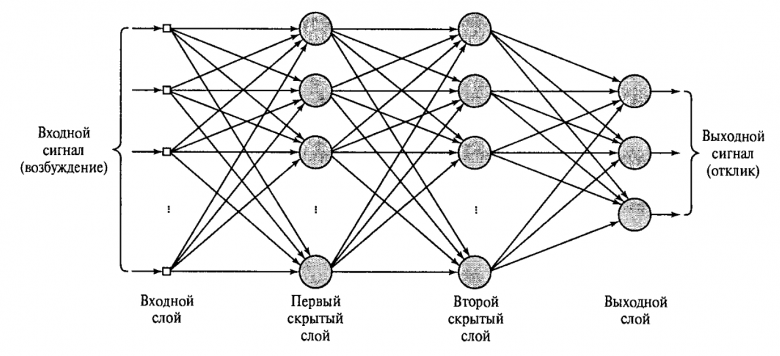
\includegraphics[width=300pt, height=150pt]{mnn.png}
	        \caption{Пример многослойной нейронной сети}
	        \label{fig:my_label}
	    \end{figure}
	\end{frame}
	
\begin{frame}{Рекуррентные нейронные сети (пример)}
	    \begin{figure}
	        \centering
	        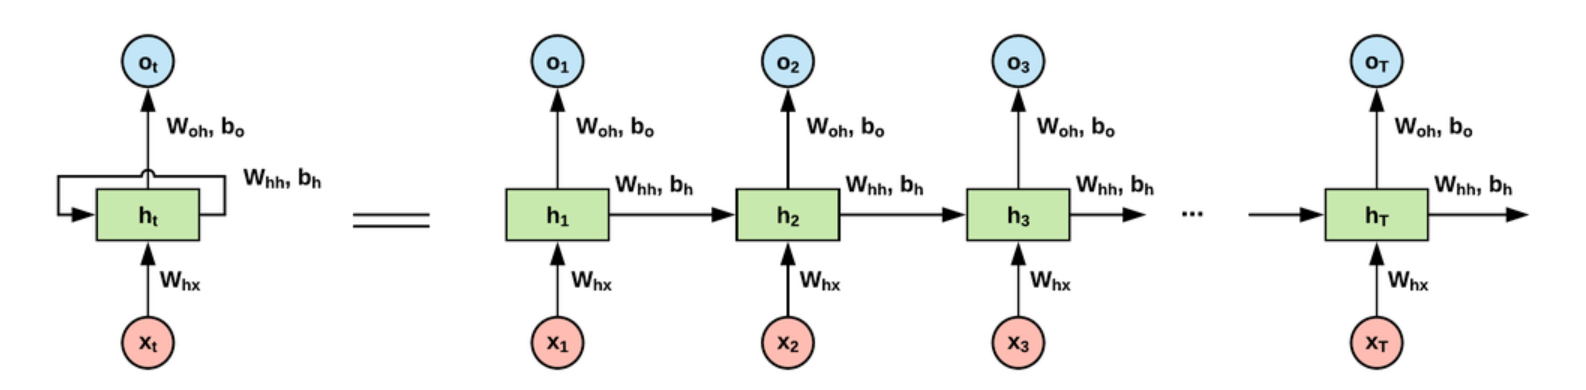
\includegraphics[width=300pt, height=80pt]{rnn.png}
	        \caption{Пример рекуррентной нейронной сети}
	        \label{fig:my_label}
	    \end{figure}
	\end{frame}


	\begin{frame}{Сверточные нейронные сети (пример)}
	    \begin{figure}
	        \centering
	        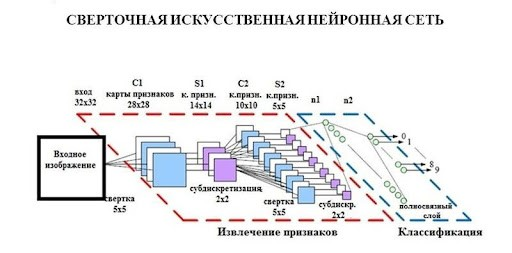
\includegraphics[width=300pt, height=150pt]{cnn.jpg}
	        \caption{Пример сверточной нейронной сети}
	        \label{fig:my_label}
	    \end{figure}
	\end{frame}
	

	\begin{frame}{Генеративно-состязательные сети (пример)}
	    \begin{figure}
	        \centering
	        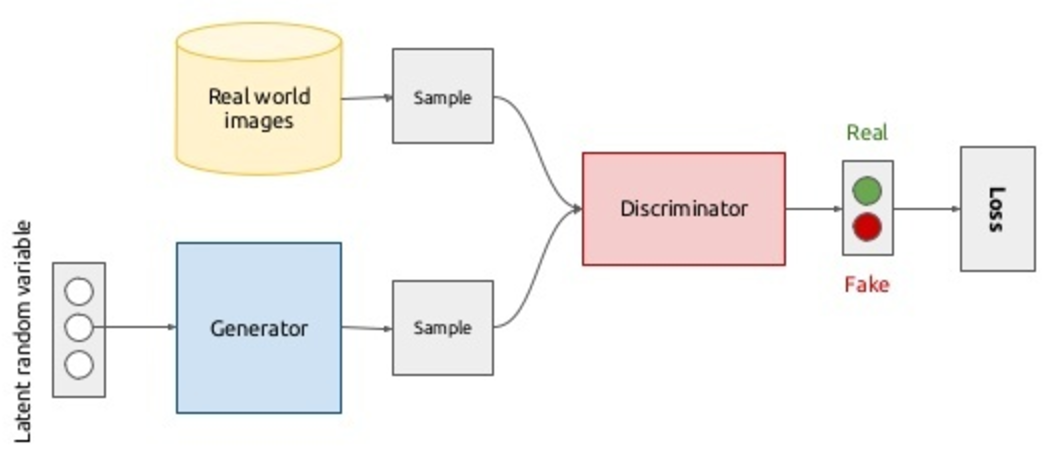
\includegraphics[width=300pt, height=150pt]{gan.png}
	        \caption{Пример генеративно-состязательной сети}
	        \label{fig:my_label}
	    \end{figure}
	\end{frame}
	
	\begin{frame}{Преобразователи (пример)}
	    \begin{figure}
	        \centering
	        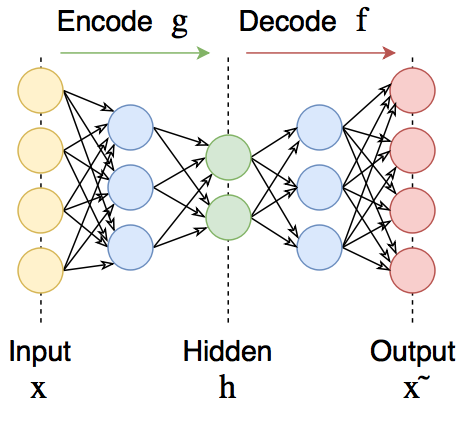
\includegraphics[width=150pt, height=150pt]{dec.png}
	        \caption{Пример автоэнкодера}
	        \label{fig:my_label}
	    \end{figure}
	\end{frame}
	
	\begin{frame}{Глубокое обучение}

    \vspace{0.5cm}
	Особенности глубокого обучения:
        \begin{itemize}
            \item большая сложность глубоких нейронных сетей;
            \item необходимость в большом количестве данных;
            \item большие трудовые, ресурсные и временные затраты;
            \item представляет собой «Черный ящик»;
            \item адаптация нейронных сетей;
            \item широкая область применения;
            \item высокая производительность.
        
        \end{itemize}
    \vspace{0.5cm}
        
	\end{frame}	

\begin{frame}
    \frametitle{Нейронные сети для изображений}

Для обработки изображений и видео наибольшей популярностью пользуются \textbf{сверточные нейронные сети}.

    \vspace{0.5cm}
	Основные преимущества:
        \begin{itemize}
            \item шаблоны, которые они изучают, являются инвариантными в отношении переноса;
            \item они могут изучать пространственные иерархии шаблонов;
            \item уменьшение количества параметров;
            \item уменьшение размерности.
        
        \end{itemize}
  
    \vspace{0.5cm}
	Используемые слои:
        \begin{itemize}
            \item сверточные слои;
            \item объединяющие слои;
            \item полносвязные слои.
        
        \end{itemize}  
        
        
\end{frame}
    
\begin{frame}
\frametitle{Сверточные слои}
	\begin{figure}[h!]
		
			\centering{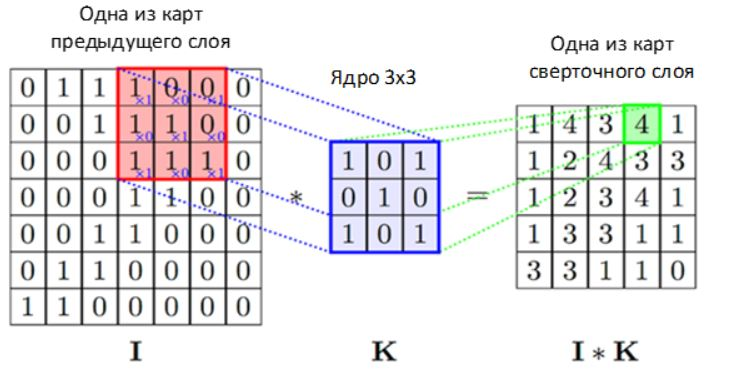
\includegraphics[width=10cm, height=5.5cm]{cnn1.JPG}}
	
	
	\end{figure}
\end{frame}

\begin{frame}
	\frametitle{Сверточные слои}
	\begin{center}
		\begin{itemize}
			\item Вход: $W_{1} \times H_{1} \times D_{1}$
			\item Гиперпараметры:
				\begin{itemize}
			 		\item $K$ -- количество фильтров
			 		\item $F$ -- размер фильтра 
			 		\item $S$ -- шаг свертки
			 		\item $P$ -- заполнение нулями
				\end{itemize}
			\item Выход: $W_{2} \times H_{2} \times D_{2}$
				\begin{itemize}
					\item $W_{2}  = (W_{1} - F + 2P)/S + 1$
					\item $H_{2}  = (H_{1} - F + 2P)/S + 1$
					\item  $D_{2} = K$
				\end{itemize}
			\item $F*F*D_{1}$ весов на фильтр, всего $F*F*D_{1}*K$ весов
			\item Далее к получившимся элементам сверточного слоя применяют функцию активации. Обычно берут $\mathsf{ReLu}(p) = \mathsf{max}(0,p)$;
		\end{itemize}
	\end{center}
\end{frame}
	
\begin{frame}
    \frametitle{Объединяющий слой}

    Объединяющий слой нейронов -- это необучаемая свёртка с щагом $\mathsf{h} >1$, агрегирующая данные прямоугольной области $\mathsf{h} \times \mathsf{h}$:

    \begin{center}
    	$\mathsf{y}[\mathsf{i},\mathsf{j}] = \mathsf{F}(\mathsf{x}[\mathsf{hi},\mathsf{hj}],\dots,\mathsf{x}[\mathsf{hi} + \mathsf{h} - 1, \mathsf{hj} + \mathsf{h} - 1])$,
    \end{center}
гду $\mathsf{F}$ -- агрегирующая функция: max, average и т.п.

\begin{figure}[h]
	\begin{center}
		\begin{minipage}[h]{0.72\linewidth}
			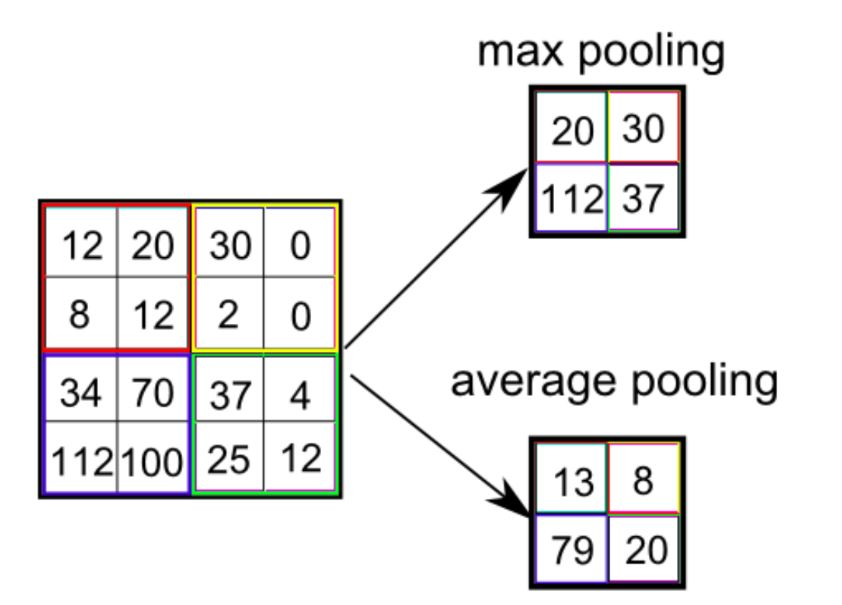
\includegraphics[width=1\linewidth]{cnn2.JPG}
		\end{minipage}
	\end{center}
\end{figure}

\end{frame}

\begin{frame}
	\frametitle{Объединяющий слой}
		\begin{itemize}
			\item Вход: $W_{1} \times H_{1} \times D_{1}$
			\item Гиперпараметры: 
				\begin{itemize}
					\item $F$ -- ширина квадратного фильтра
					\item $S$ -- шаг фильтра
				\end{itemize}
			\item Выход: $W_{2} \times H_{2} \times D_{2}$:
				\begin{itemize}
					\item $W_{2} = (W_{1} - F)/S + 1$
					\item $H_{2} = (H_{1} - F)/S + 1$
					\item $D_{2} = D_{1}$
				\end{itemize}
		\end{itemize}
		\begin{figure}[h]
	\begin{center}
		\begin{minipage}[h]{0.92\linewidth}
			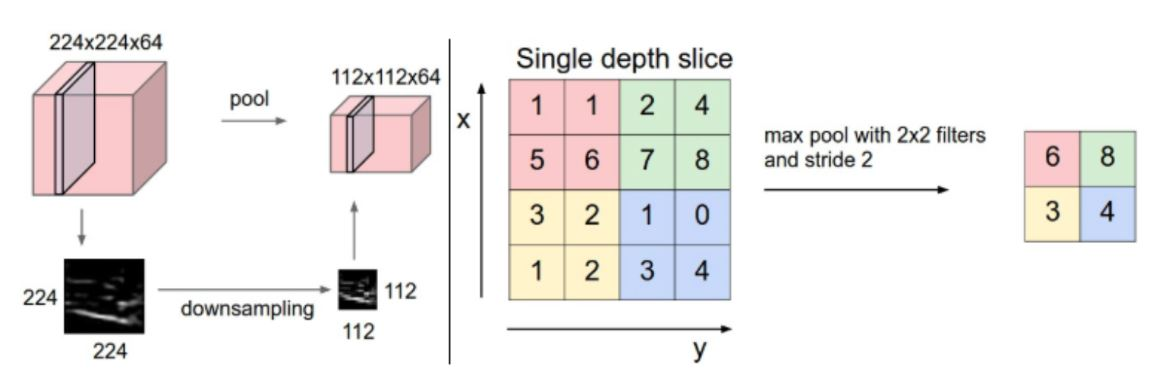
\includegraphics[width=1\linewidth]{cnn3.JPG}
		\end{minipage}
	\end{center}
\end{figure}
\end{frame}

\begin{frame}
	\frametitle{Полносвязный слой}
	Последний из типов слоев это слой обычного многослойного персептрона. Цель слоя – классификация, моделирует сложную нелинейную функцию, оптимизируя которую, улучшается качество распознавания. Вычисление значений нейрона можно описать формулой:
	\begin{center}
		$\mathsf{x}_{\mathsf{j}}^{\mathsf{l}} = \sigma(\sum \limits_{\mathsf{i}} \mathsf{x}_{\mathsf{i}}^{\mathsf{l-1}} * \mathsf{w}_{\mathsf{i,j}}^{\mathsf{l-1}}+\mathsf{b}_{\mathsf{j}}^{\mathsf{l-1}})$,
	\end{center}
	где
	\begin{itemize}
		\item $\mathsf{x}_{j}^{l}$ -- карта признаков $\mathsf{j}$ (выход слоя $\mathsf{l}$), 
		\item $\sigma()$ -- функция активации,
		\item $\mathsf{b}^{\mathsf{l}}$ -- коэффициент сдвига слоя $\mathsf{l}$,
		\item $\mathsf{w}_{\mathsf{i,j}}^{\mathsf{l}}$ -- матрица весовых коэффициентов слоя $\mathsf{l}$.
	\end{itemize}
\end{frame}

\begin{frame}
	\frametitle{Функция активации}
	 Выделяются следующие функции активации:
		\begin{itemize}
			\item сигмойда: $\sigma(z) = \frac{1}{1 - e^{-az}}$, $a \in \mathbb{R}$;
			\item гиперболический тангенс: $\sigma(z) = \frac{e^{az} - e^{-az}}{e^{az} + e^{-az}}$;
			\item softmax: $\sigma(z)_{\mathsf{i}} = \frac{e^{z_{\mathsf{i}}}}{\sum \limits_{k=1}^{K} e^{z_{k}} }$.
		\end{itemize}
	
\end{frame}

	\begin{frame}
		\frametitle{Forwardpropagation}
		Операция свертки может быть записана так, как описано на рисунке ниже.
		\begin{figure}[h]
			\begin{center}
				\begin{minipage}[h]{0.92\linewidth}
					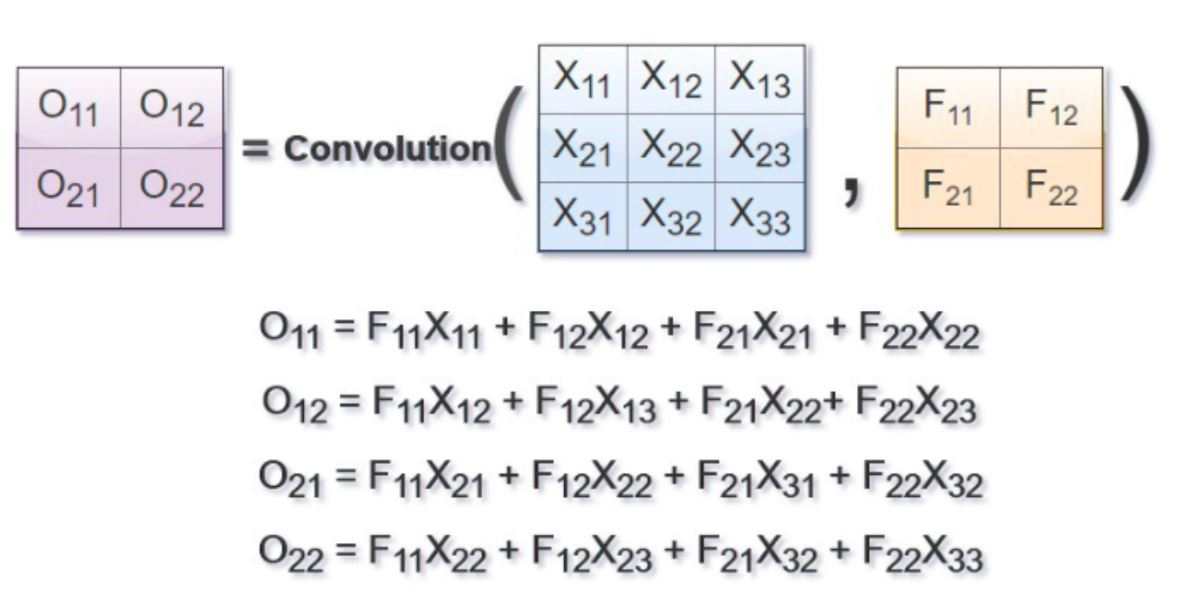
\includegraphics[width=1\linewidth]{cnn4.JPG}
				\end{minipage}
			\end{center}
		\end{figure}

	\end{frame}

	\begin{frame}
		\frametitle{Forwardpropagation}
		Теперь, чтобы вычислить градиенты фильтра $F$ относительно ошибки $E$, необходимо решить уравнения, которые можно записать в форме операции свертки.

		\begin{figure}[h]
			\begin{center}
				\begin{minipage}[h]{0.92\linewidth}
					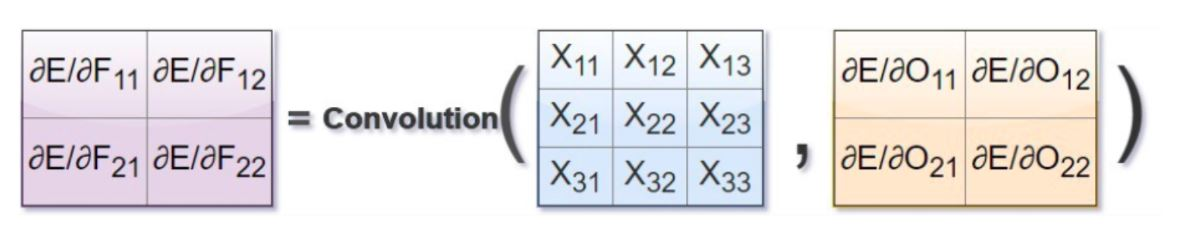
\includegraphics[width=1\linewidth]{cnn5.JPG}
				\end{minipage}
			\end{center}
		\end{figure}
	\end{frame}

\begin{frame}
	\frametitle{Forwardpropagation}
	Точно так же мы можем найти градиенты входной матрицы $X$ относительно ошибки $E$.
\begin{figure}[h]
			\begin{center}
				\begin{minipage}[h]{0.92\linewidth}
					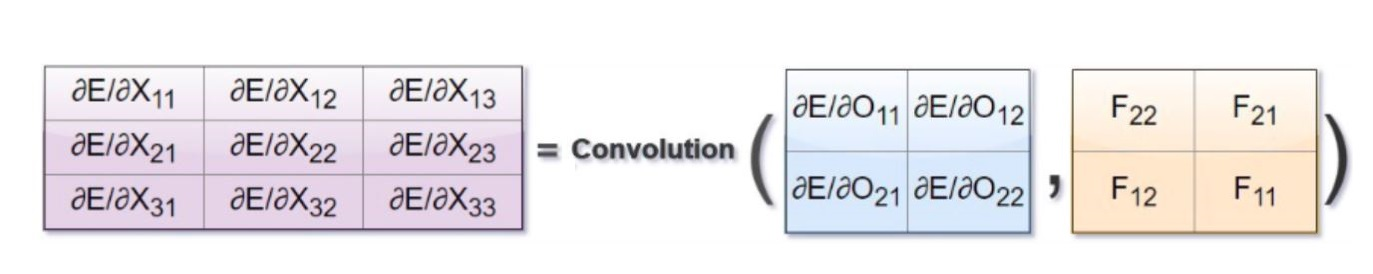
\includegraphics[width=1\linewidth]{cnn6.JPG}
				\end{minipage}
			\end{center}
		\end{figure}

\end{frame}
	

\end{document}
